%%
%  ******************************************************************************
%  * #file    Szablon_raportu_EN_Latex.tex
%  * #author  Adrian Wójcik   adrian.wojcik(at)put.poznan.pl
%  *          
%  * #commit  Patryk Kościk   koscikpatryk(at)gmail.com
%  *          Modified the template for Projekt przejsciowy purposes          
%  *          
%  * #version 1.0
%  * #date    09-Mar-2022
%  * #brief   PROJPRZEJ
%  *
%  ******************************************************************************
%%  
\documentclass[11pt, a4paper]{article}

\usepackage{SM_template}

% Wypełnijcie te dyrektywy zgodnie z waszym tematem
% \lab      -> NAZWA CZUJNIKA, np.: 'DHT22'
% \comment  -> Króciutki opis co to, np.: 'Cyfrowy budżetowy czujnik temperatury'
%

\lab{DHT-22 (AM2302)}
\comment{Cyfrowy czujnik temperatury i wilgotności otoczenia}
\author{Dawid Wasung}
\addbibresource{bib/KY-018.bib}

% Absolutny zakaz dotykania tego tutaj bo jak dotkiecie to coś jebnie
\university{Politechnika Poznańska}
\faculty{Wydział Automatyki, Robotyki i Elektrotechniki}
\institute{Instytut Robotyki i Inteligencji Maszynowej}
\department{Zakład Sterowania i Elektroniki Przemysłowej}

\nocite{*}


%%
%
% Początek dokumentu
%
%%
\begin{document}

%% Strona tytułowa %%
\mainpage{{KY-018/front}}
\newpage

\section*{Opis elementu} \addcontentsline{toc}{section}{Wstęp}
Czujnik DHT22, występujący też pod nazwą AM2302, jest cyfrowym czujnikiem temperatury i wilgotności otoczenia, lepszym następcą dobrze znanego DHT11 (AM2301). Charakteryzuje się znacznie większym zakresem i dokładnością pomiarów - w przypadku temperatury jest to od -40$^{\circ}$C do 80$^{\circ}$C (dokładność $\pm$ 0.5$^{\circ}$C), natomiast dla wilgotności zakres wynosi 0-100\% RH (dokładność $\pm$2\%). Zasilany może być napięciem 3.3V-6V, a średni pobór prądu to 0.2mA. Posiada cztery piny, z czego jedynie trzy są użyteczne - VCC, GND oraz transmisji danych. 
\vspace{0.5cm}
\begin{figure}[h!]
\centering
\begin{subfigure}{.5\textwidth}
  \centering
  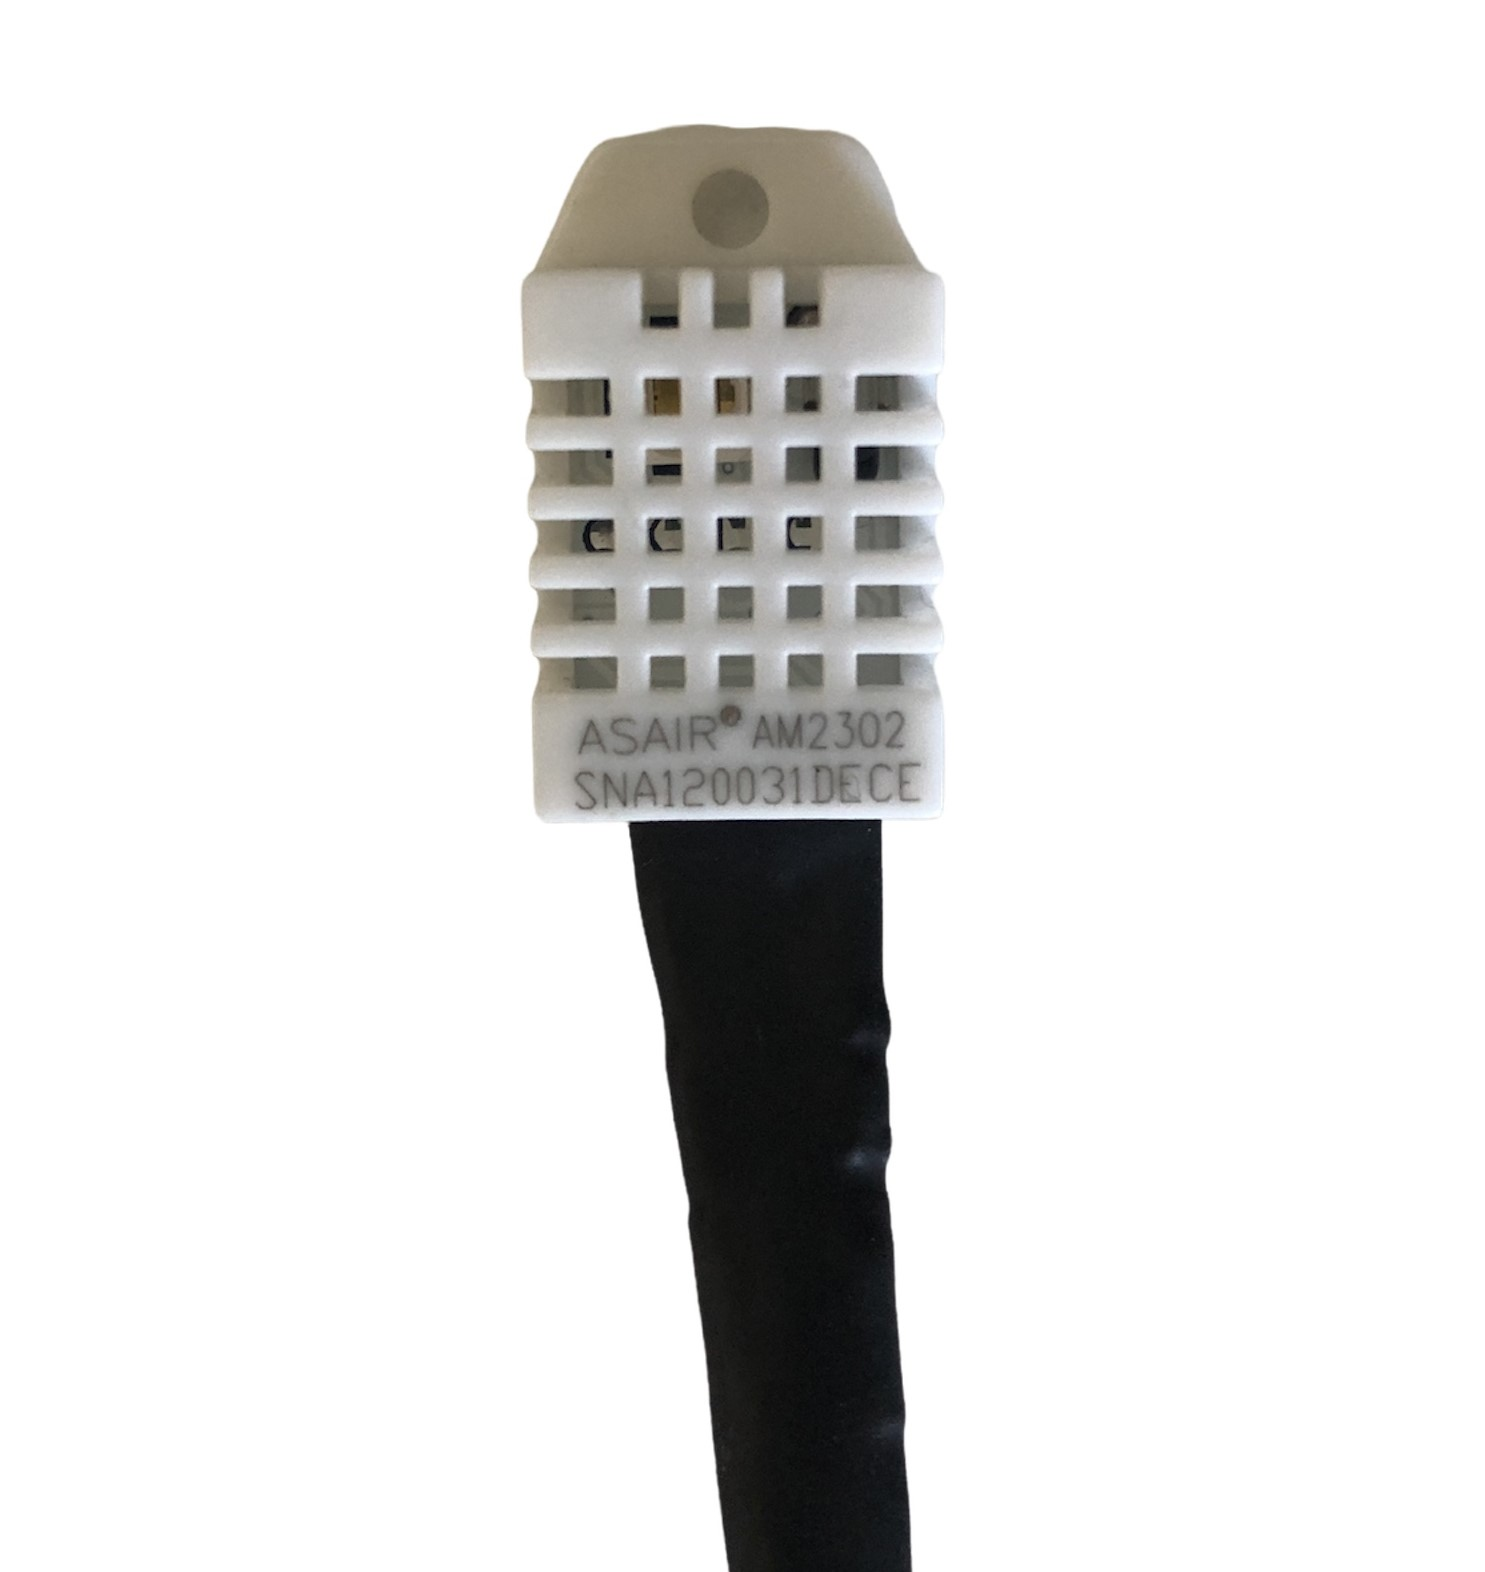
\includegraphics[width=.7\linewidth]{fig/KY-018/zdj_modułu/front.jpg}
  \caption{Wygląd czujnika}
  \label{fig:sub1}
\end{subfigure}%
\begin{subfigure}{.5\textwidth}
  \centering
  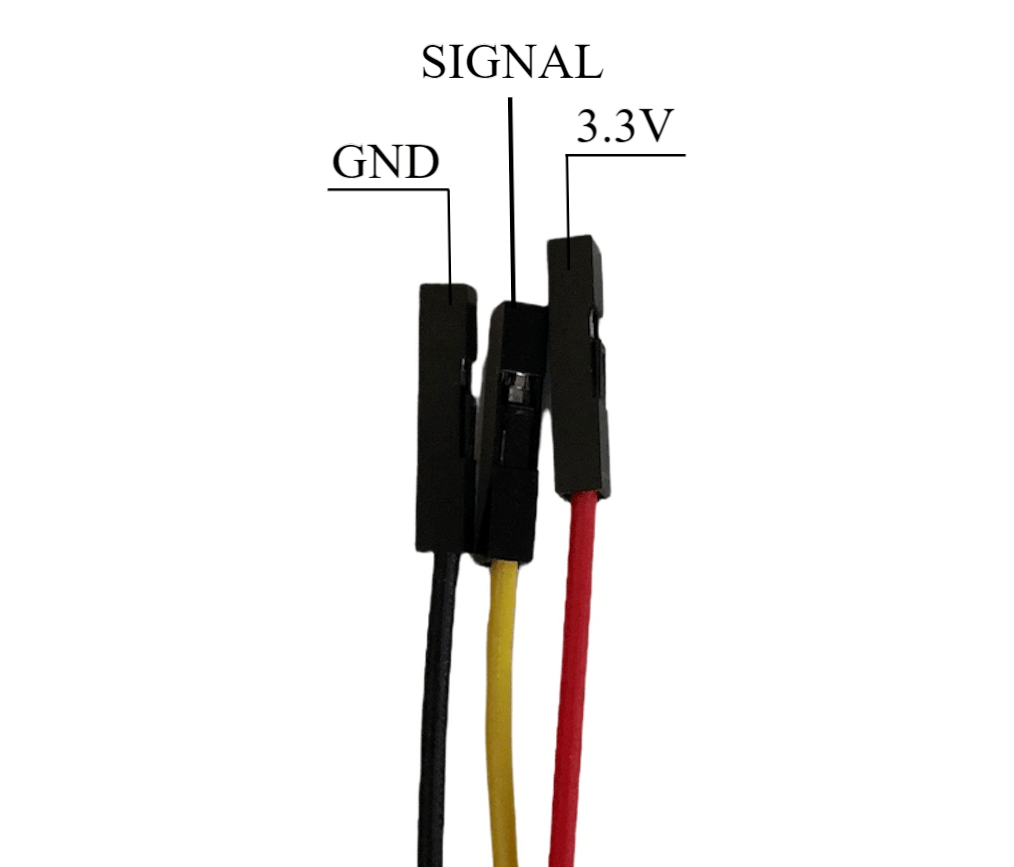
\includegraphics[width=0.86\linewidth]{fig/KY-018/zdj_modułu/kable.png}
  \caption{Wyprowadzenia}
\end{subfigure}
\caption{Wygląd oraz wyprowadzenia czujnika}
\label{fig:test}
\end{figure}

Mierzona wilgotność, to wilgotność względna (informacja o tym, ile wilgoci zawiera się w powietrzu o danej temperaturze; 100\% oznacza całkowite skroplenie się zawartej w powietrzu wody). DHT22 można zakupić w dwóch wersjach, jako zwykły czujnik lub jako moduł, do którego dołączony jest filtrujący kondensator i rezystor pull-up, które skutecznie odszumią sygnał cyfrowy. Należy pamiętać, że informacja zwrotna z czujnika składa się w sume z 5 bajtów dotyczących wilgotności, temperatury oraz bitu parzystości - w takiej sytuacji pin I\slash O musi być zmieniany na stan niski i wysoki w odpowiednich odstępach czasowych, by dopuścić do wymiany informacji.

\begin{figure}[h!]
\centering
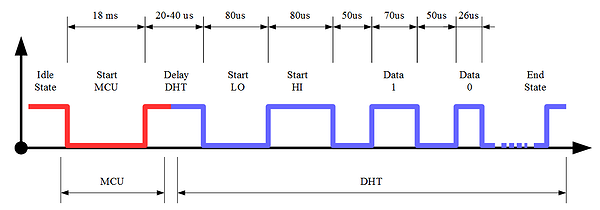
\includegraphics[width=1\linewidth]{fig/KY-018/działanie_ukladu/wykres.png}
\caption{Diagram czasowy modułu \cite{DHT:wykres}}
\label{fig:sub2}
\end{figure}

\newpage
\section*{Użycie czujnika}

Poniżej przedstawiono implementację czujnika z wykorzystaniem filtrującego kondensatora oraz rezystora pull-up.

\vspace{0.5cm}
\begin{figure}[h!]
    \centering
    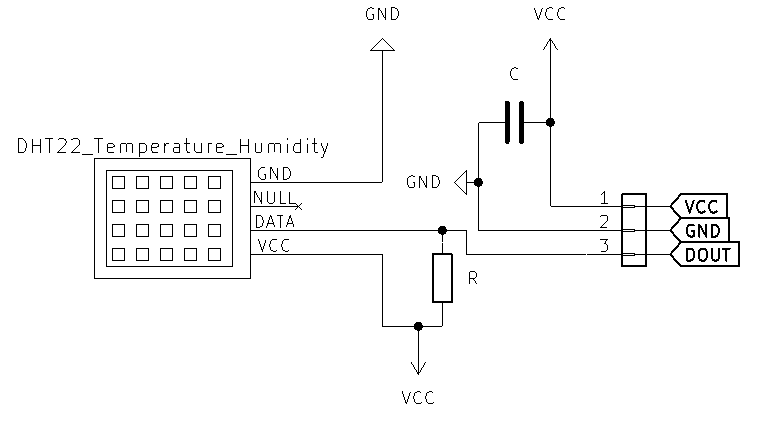
\includegraphics[width=0.8\textwidth]{fig/KY-018/działanie_ukladu/schemat.png}
    \caption{Schemat czujnika z dodatkowym filtrem}
    \label{fig:my_label}
\end{figure}

Przy programowaniu czujnika należy pamiętać o częstotliwości, z jaką DHT22 się odświeża - 1Hz, czyli co sekundę - powinno zostać zaimplementowane opóźnienie > 1s w celu poprawnego funkcjonowania.

\begin{figure}[h!]
\centering
\begin{subfigure}{.5\textwidth}
  \centering
  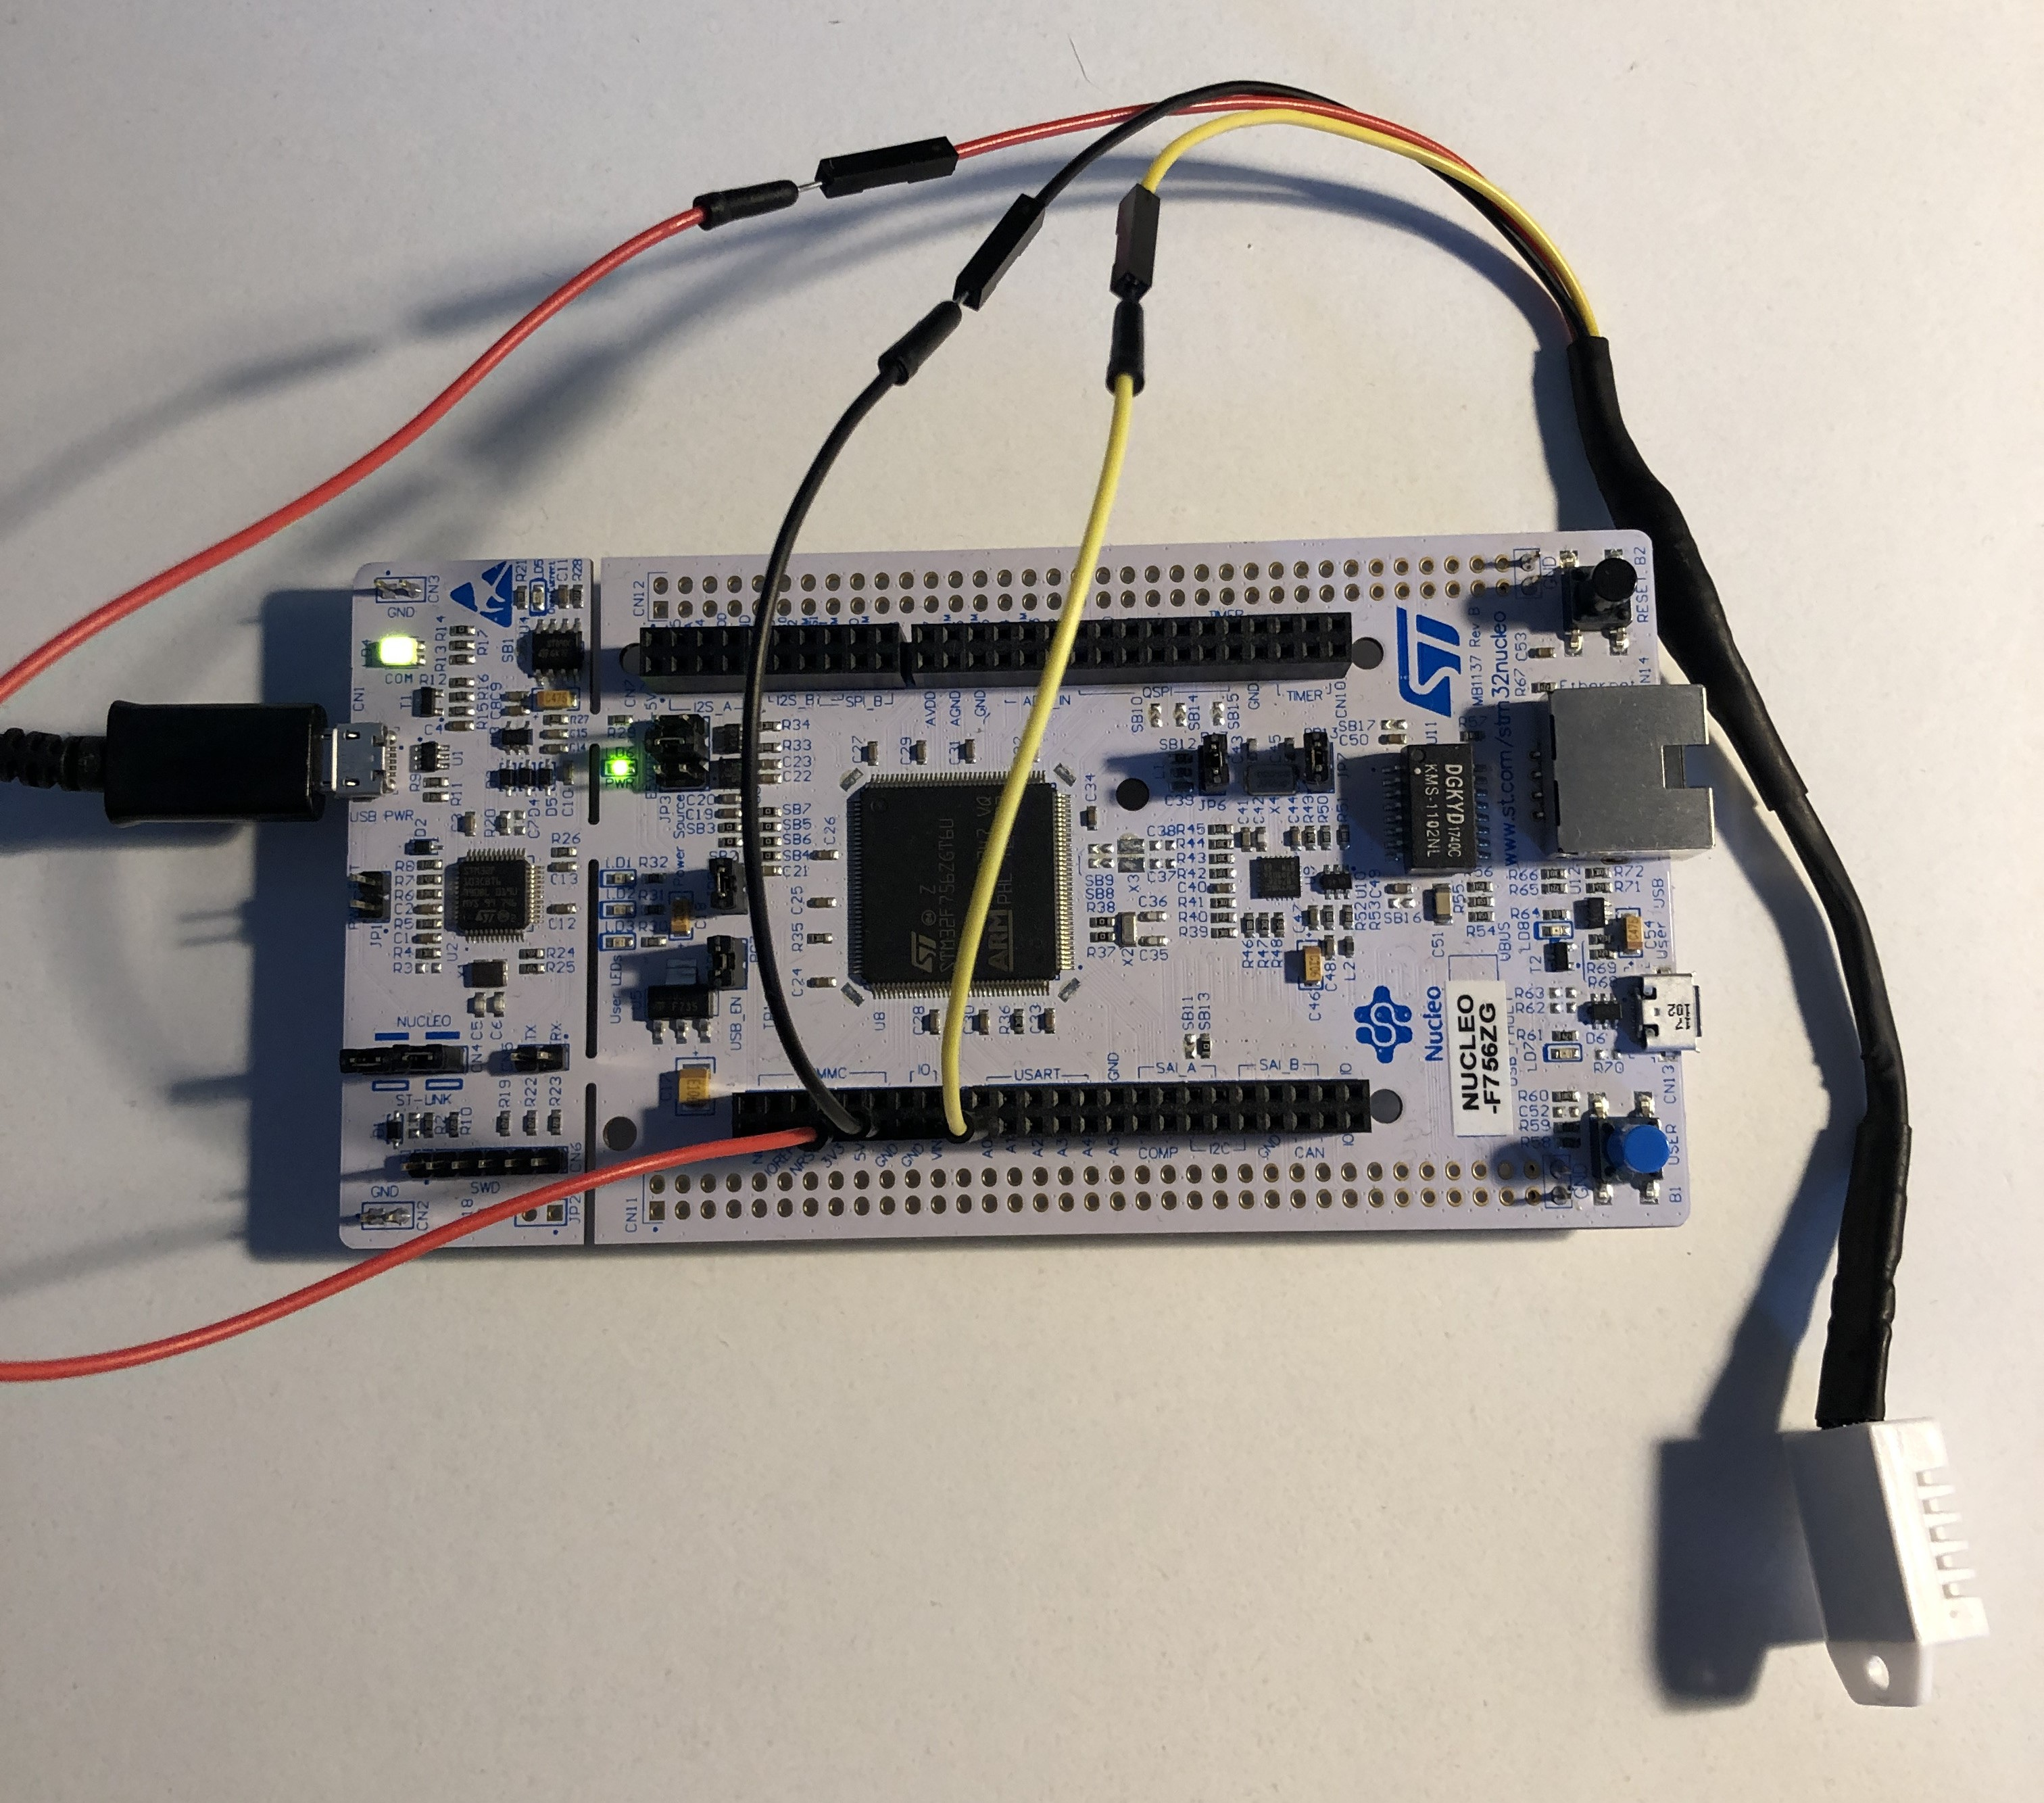
\includegraphics[width=.7\linewidth]{fig/KY-018/polaczenie_modulu/uklad.jpg}
  \caption{Podłączenie czujnika}
  \label{fig:sub1}
\end{subfigure}%
\begin{subfigure}{.5\textwidth}
  \centering
  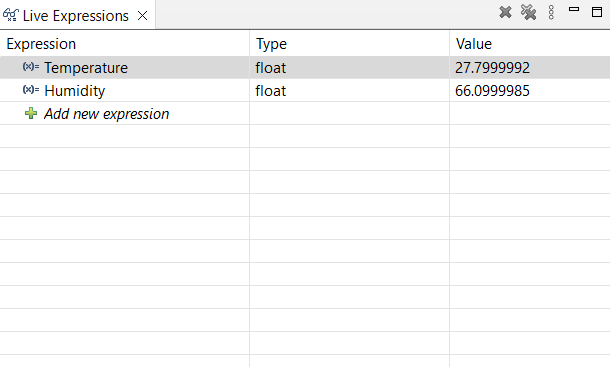
\includegraphics[width=1\linewidth]{fig/KY-018/działanie_ukladu/expres.png}
  \caption{Odczyt danych}
\end{subfigure}
\caption{Podłączenie oraz działanie czujnika}
\label{fig:test}
\end{figure}
Na Rys.4(a) zostało przedstawione najprostsze połączenie modułu z mikroprocesorem - filtr nie jest niezbędny do działania układu, natomiast poprawia jego dokładność i jakość odczytywanych informacji. Rys. 4(b) prezentuje odczyty danych z czujnika - temperatura w stopniach Celsjusza oraz wilgotność w \%.
\newline

Kod programujący czujnik, wykorzystany do opracowania instrukcji, znajduje się w materiałach dodatkowych zawartych pod koniec rozdziału.

Film prezentujący działanie układu znajduje się w suplemencie wideo

\newpage

\printbibliography[heading=bibintoc]

\end{document}